
%%%%%%%%%%%%%%%%%%%%%%% file typeinst.tex %%%%%%%%%%%%%%%%%%%%%%%%%
%
% This is the LaTeX source for the instructions to authors using
% the LaTeX document class 'llncs.cls' for contributions to
% the Lecture Notes in Computer Sciences series.
% http://www.springer.com/lncs       Springer Heidelberg 2006/05/04
%
% It may be used as a template for your own input - copy it
% to a new file with a new name and use it as the basis
% for your article.
%
% NB: the document class 'llncs' has its own and detailed documentation, see
% ftp://ftp.springer.de/data/pubftp/pub/tex/latex/llncs/latex2e/llncsdoc.pdf
%
%%%%%%%%%%%%%%%%%%%%%%%%%%%%%%%%%%%%%%%%%%%%%%%%%%%%%%%%%%%%%%%%%%%


\documentclass[runningheads,a4paper]{llncs}

\usepackage{amssymb}
\usepackage{amsmath}
\setcounter{tocdepth}{3}
\usepackage{graphicx}

\DeclareMathOperator{\fft}{fft}

\usepackage{url}
\urldef{\mailsa}\path|{m.martineau,cssnmis}@bristol.ac.uk|    
\newcommand{\keywords}[1]{\par\addvspace\baselineskip
\noindent\keywordname\enspace\ignorespaces#1}

\begin{document}

\mainmatter  % start of an individual contribution

% first the title is needed
\title{Composing HPC Packages and the Influence of Dominant Performance Characteristics}

% a short form should be given in case it is too long for the running head
\titlerunning{Composing the Dwarfs}

\author{Matt Martineau \and Simon McIntosh-Smith}
%
\authorrunning{Composing the Dwarfs}

% the affiliations are given next; don't give your e-mail address
% unless you accept that it will be published
\institute{Merchant Venturers Building, Woodland Road, Bristol, BS81UB, United Kingdom\\
  \mailsa\\
\url{}}

%
% NB: a more complex sample for affiliations and the mapping to the
% corresponding authors can be found in the file "llncs.dem"
% (search for the string "\mainmatter" where a contribution starts).
% "llncs.dem" accompanies the document class "llncs.cls".
%

%\toctitle{Lecture Notes in Computer Science}
%\tocauthor{Authors' Instructions}
\maketitle


\begin{abstract}
  In this paper we discuss the composition of scientific packages, and how this affects performance on highly parallel supercomputing hardware. We introduce three new mini-apps: Hot, Flow, and Fast, which solve heat diffusion and hydrodynamics, and perform parallel FFTs to solve Poissons equation. The mini-apps represent three of the seven Dwarfs of parallel programming, and have been developed with the purpose of evaluating the impact of coupling those algorithms together.

  Although much research has been performed that evaluates the performance profile of the seven Dwarfs, production applications rarely utilise only a single package for solving a scientific problem. We start by presenting a motivational discussion of the relevant Dwarfs, considering their invidual performance characteristics and which of those characteristics are dominant. Following this we present performance results of coupling Hot, Flow, and Fast together, using them to solve test problems on modern hardware.  

  The paper ends with a discussion of some of the most important performance issues that we can forsee when coupling applications together, motivating a stream of future work in the area.

  \keywords{performance portability,mini-apps,high performance computing,openmp 4}
\end{abstract}

\section{Introduction}

A great amount of work is being devoted to understanding how scientific production applications will be ported to run on modern supercomputers. Some context of the challenges currently faced by the community is presented to demonstrate the importance of this research. 

\subsection{The Use of Mini-Apps to Optimise for Modern Architectures}

To meet power demands and continue to grow the performance capabilities of supercomputing resources, a continual diversification of architectures has been essential. This has brought significant complexities for scientific applications developers, necessitating improvements in programming environments and the optimisation of algorithms. Due to the extent of the task, it is now essential that computer scientists are involved in the process, which has lead to a surge of co-design projects. In particular, many optimisation projects are being performed with proxy applications, or mini-apps, such that the lessons can be prototyped in collaboration between scientists and computer scientists.

A great many studies have been performed that have used mini-apps to investigate key problems such as application performance, portability, scalability, and fault tolerance. In spite of this, the research does not generally make a link between the optimisations seen for those miniaturised proxy applications and full scale production applications.

%It is considered an onerous and complicated task to program GPUs and until recently there has been little traction within the community to port existing large-scale applications, even though some of the largest supercomputers in the world, for instance Titan, include both CPUs and GPUs. We have shown in our previous research that GPUs can be programmed effectively, in most cases, using existing programming models. We have shown that productivity can be an important deciding factor in the choice of programming model, and further showed that directive-based models can offer a highly productive interface, that can be portable given good implementations, whilst not significantly sacrificing performance.

\subsection{Extending the Single Mini-App Focus}

This paper is a window into a set of work that is attempting to extend the success of mini-apps for evaluating modern architectures and programming environments. It is essential that the community is mindful of the purpose of mini-apps, which is to discover optimisations that have real world impact. Our aim is to begin to capture the features of production scientific codes that have been yet unexplored with mini-apps, to improve the validity of future performance investigations. 

Much of the mini-app optimisation focus has been limited to individual applications which have, in general, performed well on modern hardware, using a range modern parallel programming models. Up until this point the individual mini-apps have failed to expose some important aspects of large-scale scientific applications, in that they are isolated instances of algorithms that do not encapsulate the multi-package hierarchies that scientists are truly interested in seeing results for.

In order to limit our focus to the most important algorithms that might be encountered within scientific production codes, we will follow the seven Dwarfs of parallel programming. In the 2006 View from Berkely paper \cite{Asanovic2006}, a number of important classes of parallel algorithm were discussed and categoried as parallel programming Dwarfs. Each of the Dwarfs exposes a diverse computational and communicational pattern and can encompass many of the algorithms you are likely to see in production scientific applications.  

Their paper eluded to the necessity for those Dwarfs to be composed together and investigated as coupled application. Our intention is to use a new suite of mini-apps, tailored for composition, to expose the dominant performance characteristics when combining multiple packages, as would be seen in a common scientific production application. Each mini-app represents one of a subset of the Dwarfs, and we plan to consider all of the Dwarfs in future research.

We recognise that many of the issues we discuss or uncover will have been discovered by application developers or performance engineers attempting to combine multiple packages together in the past. However, it can often be challenging to generalise approaches from specific use cases, which is one of the benefits of mini-apps, where a general strategy can be employed and discussed. Ultimately, it is essential to the relevance of results obtained by mini-apps that such features are considered alongside other performance studies. 

\section{Contributions}

This research is primarily focussed upon discussing the implication of composing a subset of the parallel application Dwarfs, and we present a number of important contributions in order to support the discussion:

\begin{itemize}
  \item We have developed three mini-apps that serve as proxy applications for important scientific algorithms. An FFT solver for Poisson equations (Fast), a heat conduction application (Hot), and a fluid dynamics application (Flow).

  \item We present results for those algorithms in isolation on some modern supercomputing architecture: an NVIDIA K40m, an Intel Xeon Phi Knights Landing (KNL) processor, an IBM POWER8 CPU, and a Intel Xeon Broadwell.

  \item We naively couple the Hot, Flow, and Fast mini-apps together to demonstrate their composed performance profiles.

  \item We offer insights into the issues and opportunities that might be experienced when composing algorithms that goes beyond the scope of our current experiments.

\end{itemize}

\section{Background}

In this section we will discuss the general composition of packages, and then present some basic details about each application, including a description of the numerical method and parallelisation strategy. To ensure a clear discussion, we will explain the initial development of each application prior to discussing our efforts to couple them together. This means that we will explain how each application was optimally developed, but with the caveat that this would likely have to change once coupling was required. We did not actively consider the coupling during the up-front development of each application, instead opting to choose the best strategy for each application in isolation.

\subsection{Composition of Dwarfs}

It would be possible to compose packages from any of the domains within science and engineering, but an aim of this research was to use canonical algorithms that can act as proxies for wider classes of application. In this paper we have chosen to continue on from the work discussed by Asanovic et al. \cite{Asanovic2006}, who outlined a number of Dwarfs, each of which describes a different computational class that features in modern supercomputing applications. Selecting algorithms that strongly correlate to the characteristics of an individual Dwarfs will offer general insights that can be applied to the wider field.

Each of the Dwarfs has a unique set of computational and communicational characteristics that mean that they expose different requirements of modern computing hardware. While many of those characteristics have been analysed and optimised heavily on existing architectures, we intend to uncover the extent to which those classes can co-exist within an application. At this stage we will re-iterate that that the majority of production applications that solve significant scientific problems will require packages encompassing a number of the classes described by the Dwarfs.

The Dwarfs cover broad families of algorithms, each of which encapsulates a subset of possible performance characteristics, with some overlap of characteristics amongst the Dwarfs. An aim of this research is to expose some dominant performance characteristics, as we hypothesise that there will be an unequal weighting of the importance of those characteristics. 

The Dwarfs that we consider in this paper are:

\begin{itemize}
  \item \textbf{Spectral Methods} - \textit{Fast}: A Fast Fourier Transform solver for Poisson's equation (Section \ref{sec:fast}).
  \item \textbf{Sparse Linear Algebra} - \textit{Hot}: An heat diffusion application, that uses a Conjugate Gradient linear solver (Section \ref{sec:hot}).
  \item \textbf{Structured Grid} - \textit{Flow}: A Lagrangian-Eulerian hydrodynamics application that uses an explicit 5 point stencil (Section \ref{sec:flow}).
  %\item \textbf{Monte Carlo} - \textit{Bright}: A time-dependent Monte Carlo neutral particle tracking application that tallies energy depositions (Section \ref{sec:bright}).
\end{itemize}

We will present the results of coupling Hot 2d with Flow 2d, and Hot 2d with Fast 2d. To support this we also discuss the potential difficulties that we anticipate will arise when composing the other Dwarfs together. 

It would be possible to end up with large spaghetti applications when composing multiple packages together, which would dilute the merits of using mini-apps. We have made every effort to ensure that the applications we develop for this purpose are simple while expressing the correct performance profiles, so that the agility of the individual mini-apps will still apply when composed. It is not our intention to introduce ground-breaking accuracy or methods into our applications.

\subsection{Fast - Fast Fourier Transform for Poisson's Equation}

\label{sec:fast}

The Fast Fourier Transform (FFT) is an important algorithm to a number of scientific and engineering domains, and there exists extensive literature regarding optimisation of parallel FFTs \cite{}. As part of this research we have developed a highly simplified FFT mini-app, which solves Poisson's equation. The primary reason for choosing this particular approach is not scientific relevance, rather that it will result in verifiable outputs, while still capturing some important performance characteristics of the Spectral class of algorithms.

We are currently relying on the optimised Intel MKL library version of the one dimensional FFT, and we then parallelise that manually using MPI. Our initial assumption is that the implementation of the FFT solve would be less important to the performance than the choice of decomposition strategy, given that the FFT operation is notoriously bound by the \textit{'All-to-All'} communication of data among processes \cite{}.

%Prior to our experimentation, we anticipated that the inclusion of an FFT package within a multi-package application would likely result in conflicts over the optimal domain decomposition. We have observed similar issues with domain decompisition conflicts for wavefront parallelism, making this pattern of great interest.

\subsubsection{Fundamental Method}

Following on from the discussions in Gholami et al. \cite{}, we utilise the FFT to solve Poisson's equation for some dependent data passed to the solver. 

\begin{align}
  \frac{d^2\phi}{dx^2} = \epsilon(x, y) \\
  \fft(\epsilon) = \hat{\epsilon} \\
  \hat{\phi_{i,j}} = \frac{\hat{\epsilon_{i,j}} dx^2 }{4 - \omega^i - \omega^{-i} - \omega^{j} - \omega^{-j}} \\
  \fft^{-1}(\hat{\phi}) = \phi
\end{align}

The solve phase calculates and FFT along the $x$ and $y$ axes of $\epsilon$, before solving the equation in Fourier space and performing an inverse FFT to return the solution $\phi$. With this current approach we are limited to periodic boundary conditions, and we plan to extend this to incorporate other boundary conditions in the future. 

The arithmetic requirement of this package is low and the algorithm is generally straightforward, especially when compared to Flow, which requires a cohesion between many numerical methods. Maintaining a simple algorithm means that we will be able to extend this application more easily to 3d in the future to compare different decompositions.

\subsubsection{Parallelisation}

In order to parallelise the FFT's it is necessary to perform a matrix transposition as part of each of the FFTs, which requires packing buffers, performing All-to-All communications with MPI, and then locally transposing the data. Due to the fact that we are performing an FFT before the solve, and then a subsequent inverse FFT, it is possible to reduce the number of transpositions from four to two, saving on the number of All-to-All communications.

The parallel decomposition of the FFT operation is architecture dependent, and in particular varies depending on how many computational elements the problem will be executed on. In the 2d implementation you are limited to a one dimensional decomposition, either row-wise or column-wise, and the parallelism is therefore limited by the problem dimensions \cite{}. The reason for this restriction is that each process has data dependencies along each axis, and so tiling would greatly increase the amount of All-to-All communication required. 

A 3d port of the application is imminent and will allow for greater flexibility, as the problem can be decomposed using either slabs or pencils. While the decomposition of the FFT can be easily solved and optimised for particular architecture in isolation, the issue is particularly important when composing an FFT package with other packages, as different decompositions might negatively impact on the performance of the whole application leading to a larger search space of decisions when optimising an application.

\subsection{Hot - Heat Conduction via a CG Solver}

\label{sec:hot}

We have developed a simple conjugate gradient (CG) solver that implicitly solves the heat conduction equation. We do not precondition the problem, and utilise a standard iterative algorithm. The problem is memory bandwidth bound, until communication costs overwhelm during strong scaling. The problem is also well studied from a HPC optimisations perspective with a number of mini-apps solving the problem, and the HPCG benchmark now being actively used to benchmark supercomputers \cite{}.

\subsubsection{Fundamental Method}

Heat conduction in two dimensions can be specified as follows:

\begin{align}
  \frac{\partial u}{\partial t} - \alpha (\frac{\partial^2u}{\partial x^2} + \frac{\partial^2u}{\partial y^2}) = 0 \\ 
  \alpha = \frac{k}{\rho c_p} \\
  u^n_{i,j} = u^{n+1}_{i,j}
\end{align}

Where $u$ is the temperature, $\alpha$ is the thermal diffusivity, $k$ is the thermal conductivity, $\rho$ is the density, and $c_p$ is the specific heat capacity. As you can see from equation (7), this particular form of the equation requires an implicit solve. The conjugate gradient method is an iterative method that descends towards a solution using conjugate vectors. To calculate the edge centered densities from the cell centered values on the mesh, we simply use the arithmetic mean.

\subsubsection{Parallelisation}

The best decomposition for this mini-app is regular cartesian, minimising the surface area to volume of each rank to reduce communication overheads. In terms of boundary conditions we selected reflective, as this was simple, and improves the verifiability of the results. The algorithm does not expose any load imbalance, and nearest neighbour halo exchanges are performed each timestep. At each iteration two scalar values, $\alpha$ and $\beta$, are calculated, which need to be distributed amongst all of the ranks. The implication is that each iteration requires two calls to MPI\_Allreduce, an obvious performance bottleneck at scale. 

As each of the core kernels contains some simple sparse linear algebra operation, such as a dot product or sparse matrix-vector multiply, it was straightforward to parallelise with OpenMP and CUDA, given the extent of the data-parallelism exposed by the algorithms.

\subsection{Flow - Fluid Dynamics via Lagrangian-Eulerian Flux Calculations}

\label{sec:flow}

The Flow mini-app is a Lagrangian-Eulerian hydrodynamics solver that is staggered in space and time. Although the mini-app is significantly larger and more complicated than our other new mini-apps, the resulting code is also significantly faster, as explicit stencil methods are particularly efficient in general.

\subsubsection{Fundamental Method}

The Lagrangian-Eulerian algorithm takes Euler's equations and explicitly solves them on a structured grid. The application uses simple smoothing to introduce artificial viscosity, with shock heating accounted for as part of the mechanical work update. For the mass flux calculations, a Van-Leer flux limiter is used to maintain a monotonic profile at shock boundaries, and slope-limited second-order interpolations are performed for energy and momentum to ensure monotonic behaviour for all dependent variables \cite{}.

Directional splitting is used in order to make the application two-dimensional, with the leading dimension switched each timestep, in order to maintain symmetry of the solution. Our explicit timestep control limits the timestep based on the CFL condition, stopping sound waves travelling further than a single cell per timestep, accounting for the additional spreading that occurs due to the artificial viscous stresses \cite{}. We have made the algorithm second order in time by interpolating our velocities half a timestep upstream for the advection stages.

As with the heat condution application, the boundary conditions we chose for this application are reflective, which particularly useful for tracking conservation to verify the results.

\subsubsection{Parallelisation}

As with the heat conduction application, the algorithm does not have any inherent load imbalance, and only requires nearest neighbour communication of halo regions. The explicit nature of the algorithm means that multiple kernels are invoked in order, and the independent kernels are inherently data parallel, allowing them to be easily threaded for CPU and GPU.

%\subsection{Bright - Monte Carlo Particle Transport}
%
%\label{sec:bright}
%
%Our transport application uses a Monte Carlo particle tracking method, making it quite different to the other two algorithms. Our initial effort split the problem into batches of particles, each of which had an individual history that was followed in a time-dependent manner. 
%
%A major aspect of the application is the data structure used to describe particles. Given that we did not have prior experience with this particular algorithmic class, we were not exactly sure which of the potential approaches would end up being the most performant, so we explored the space and performed some testing which we describe in detail later. Ultimately, we described a single particle using a data structure that contains the particle's position in space, direction, energy, and initially tracked the particles location by cell on the mesh.
%
%Our simple tracking procedure would maintained several running timesteps to different event types: (1) a Collision event, which is where the particle would either change direction or have some of its weight absorbed, (2) a Facet event, where the particle reached the boundary of a cell or zone, and (3) a Census event, where the particle reached the end of the current timestep. Of course, the census events for the application in isolation were simply set to some small constant size, with the intention for this timestep to be later controlled by the requirement of the CFL condition exposed by the fluid dynamics simulation.
%
%In order to determine if a Collision event has occured, we perform a lookup to cross sectional data taken from the ENDF database. In our particular approximation, we only consider absorption and scattering, ignoring any contributions due to fission. In order to reduce the overall variance of the simulation, we extend the lifespan of particles by giving them a weight, and reducing this weight each time an absorption event occurs, rather than declaring them as dead particles. Once the weight has reduced past a certain point, or the particle has reached a low enough energy, we will only then consider the particle to be dead.
%
%When a Collision event occurs and the result is a scattering of the particle a random number is generated to determine the angle of scattering, and this is also used to determine the level of energy dampening that occurs using well known relations \cite{}.
%
%To perform facet intersection checking, we are able to leverage the simple geometry of the structured grid to calculate the new direction using a simple method of our own devising. We first check which of the edges would be hit first if the particle were travelling at the same speed but only along a single axis, and use this to solve the system of equations that arises to determine the intersection point. We have considered that this might not be optimal, and doesn't generalise beyond the basic geometry presented by our structured grid case.
%
%In terms of boundary conditions we did select reflective at this stage, as this made it easier to track some conservation in the system, and matches the approach taken with the hydrodynamics solver, although we did recognise that it would likely be more representative if the boundary conditions were transmissive.
%
%Of course, all of this requires a sufficient random number generator with a large period. In order to fulfil this requirement we leveraged an existing lightweight Mersenne-Twister algorithm, to generate random numbers for the whole system.
%
%\subsubsection{Parallelisation}
%
%Unlike the other two applications, the Monte Carlo method exposes some load imbalance. There are a number of approaches to improving this problem, and we explored some of them to select the best for our particular set of requirements. 

%In terms of parallelising the algorithm there were several factors to consider, for instance it is important to maintain good data locality in particular for vectorisation on CPUs and coalescense on GPUs. Our initial strategy was to perform a coarse-grained parallelism, splitting the particles into batches in order for them to be processed in parallel. Of course this has implications in terms of the memory layout as the particles are tracked through space.

\section{Performance Characteristics of the Mini-Apps}

Although the Dwarfs imply some high-level classification of algorithms, we believe it is important to consider all of the characteristics of the particular algorithms we have chosen. Some of the most important performance characteristics of the mini-apps are listed in Table \ref{tab:perf-char-mini-apps}.

\begin{table}[h]
  \begin{center}
    \begin{tabular}{cccc}
      \hline
      \textbf{Property} & \textbf{Hot} & \textbf{Flow} & \textbf{Fast} \\
      \hline
      \textit{\textbf{Nearest Neighbour Communciation}} & Yes & Yes & No  \\
      \textit{\textbf{Iterative}} & Yes & No & No \\
      \textit{\textbf{Mesh-based}} & Yes & Yes & Yes \\
      \textit{\textbf{Stencil-based}} & Yes & Yes & No \\
      \textit{\textbf{All to All Communications}} & Yes & No & Yes \\
      \textit{\textbf{Memory-Bandwidth Bound}} & Yes & Yes & No \\
      \textit{\textbf{Multiple Optimal Decompostions}} & No & No & Yes \\
      \textit{\textbf{Load Imbalance}} & No & No & No \\
    \end{tabular}
  \end{center}
  \caption{Performance characteristics of the four mini-apps.}
  \label{tab:perf-char-mini-apps}
\end{table}

We have seen in previous work which of those characteristics matter to the individual application, such as \textit{Memory Bandwidth} for indiviual application performance and \textit{All-to-All} communications for scalability. Our intention is to investigate how the computational and communicational profiles of those applications interact with eachother when packages are composed and make some commentary about the dominant performance characteristics.

We can pre-emptively assess some of the likely effects that running multiple mini-apps at once lead to. We would expect that there could be an impact on cache utilisation, and a generally increased memory footprint, while some state could be shared potentially improving the overall performance. Table \ref{tab:perf-char-mini-apps} lists some of the key performance characteristics of the applications that we investigate in this paper. 

Some communication costs could be saved if variables could be communicated once for all applications, during the \textit{Nearest Neighbour} or \textit{All to All communications}, for instance. We do no expose any \textit{Load Imbalance} as part of our suite of applications, but are currently in the process of develop Bright, which is a Monte Carlo neutral particle tracking application, that we expect to suffer from significant load balancing issues. As two of the applications are \textit{Memory Bandwidth} bound, it might be possible to overlap the costly memory access delays with independent computation from other applications. It is also possible that data structures between the individual applications will require some form of transformation, which we expect to have a major influence on performance. 

\section{Coupling}

As the mini-apps and their composition routines were developed by computer scientists interested in the evaluation of performance profiles on modern architecture, the exact physical solution to the test problems is not important. However, the individual applications have been carefully validated to ensure that they accurately solve the chosen test methods.

We could see two different approaches to coupling the applications, the first of which involves directly coupling their constituent equations and solving the whole system at once. This approach has two important drawbacks: (1) the complexity of this approach is significant, especially considering that we plan to extend this project into a suite of seven algorithms, and (2) reducing the algorithms into a single solve would not capture the potential difficulties of coupling distinct packages together.

In general we do not consider the coupling approach to be necessarily valid from a scientific standpoint. Our intention is simply to model a simple data dependency between the applications, that leads to them having to rely on shared meshes and decompositions. It is likely important future work to investigate the impact of performing more detailed couplings, but would require complex domain-specific knowledge far beyond the scope of our research. A simple example of how we have handled coupling can be seen in Figure \ref{fig:hot-flow-flow}, where the initial conditions of density ($\rho$), energy ($\epsilon$), and momentum ($\rho u$ and $\rho v$) are passed in to start the cycle. Once the Flow phase is complete, the density and energy are passed to Hot, which then solves the timestep for temperature $\mu$, and passes back the updated energy to start the cycle again.

\begin{figure}
  \centering
  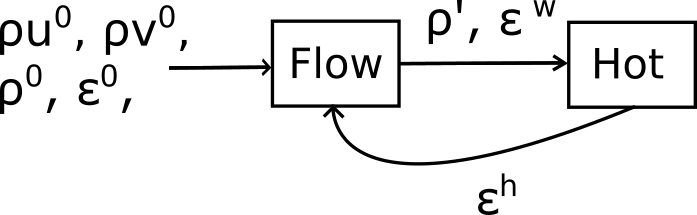
\includegraphics[width=0.6\linewidth]{hot-flow-flow}
  \caption{The data dependency of our coupled Hot and Flow applications.}
  \label{fig:hot-flow-flow}
\end{figure}

Composing Fast 2d and Hot 2d together was more challenging than with Hot 2d and Flow 2d, as the standard decompositions were different for each applications. For the sake of simplicity we constructed an artificial dependency between the packages, where a single dependent variable is passed through each of the solvers.

\section{Performance Analysis of Compositions}

Although we had some preconceptions regarding the likely effects of composing particular applications, we were objective in our assessment of the combined performance. In particular, we took time to validate that our assumptions were correct wherever possible, and have performed experimentation of a range of different platforms to observe whether there were any unexpected architectural influences.

\subsection{Experimental Setup}

Each of the mini-apps has been optimised using modern techniques from years of research optimising similar algorithms. We expect that the individual performance of the application is close to optimal, without sacrificing portability through the use of non-portable programming techniques. For each of the applications we have developed ports to OpenMP 3.0, OpenMP 4.0 and CUDA.

\begin{table}[h]
  \begin{center}
    \begin{tabular}{l|c|c}
      \hline
      \textbf{} & \textbf{Mem BW} & \textbf{FLOPS}  \\
      \hline
      \textit{\textbf{Intel Xeon E5-2699 v4 @ 2.20GHz (22 core)}} & 62 GB/s & ??? G/flops \\
      \textit{\textbf{Intel Xeon Phi 7210 (64 core)}} & 450 GB/s & ??? G/flops \\
      \textit{\textbf{NVIDIA K20X Kepler}} & 180 GB/s & ??? G/flops \\
      \textit{\textbf{NVIDIA K40m Kepler}} & 190 GB/s & ??? G/flops \\
    \end{tabular}
  \end{center}
  \caption{The devices used in this performance analysis.}
  \label{tab:hardware}
\end{table}

We will state the compilers and toolkit versions used as and when we present relevant data, and the devices we execute on can be found in Table \ref{tab:hardware}. The devices we have chosen are present in many of the largest and most active supercomputers in the world, which we hope will strengthen the relevance of any findings.

As the heat diffusion solver is iterative, it is possible to have some variance in the number of iterations performed based on the problem dimensions and initial conditions. In order to make the results more comparable across devices and between experiments we fixed the iteration count.

\subsection{Hot 2d + Flow 2d}

Given the performance characteristics we have described for both Hot and Flow, we couldn't predict any significant issues that might arise when coupling them. We are presenting two applications that have been developed from scratch, and so we provide individual scaling results to demonstrate that each application performs to an acceptable level. 

\subsubsection{Scaling}

We provide the scaling of composing the two packages into a single application.

\begin{figure}
  \centering
  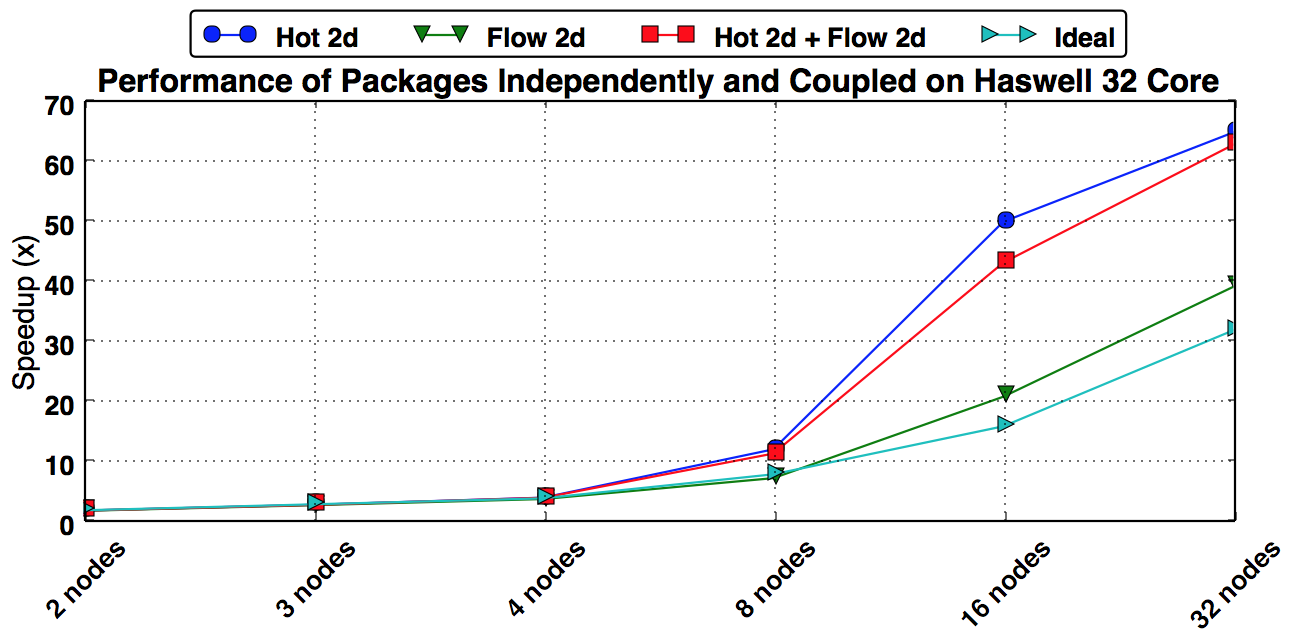
\includegraphics[width=1.0\linewidth]{cpu_results}
  \caption{Scaling Hot 2d, Flow 2d, and Hot 2d + Flow 2d on multiple nodes containing dual socket 22 core Broadwell CPUs.}
  \label{fig:scaling-hot-flow-broadwell}
\end{figure}

As can be seen from Figure \ref{fig:scaling-hot-flow-broadwell}, the results of scaling the application across 32 nodes of dual socket 22 core Broadwell CPUs demonstrate a consistent performance profile. Each of the applications beat the ideal scaling performance over a single node due to the improved utilisation of cache that occurs as the problem is decomposed into smaller chunks. There is a noticeable gap in the scaling of the two packages at 16 nodes, that greatly reduces by the time that 32 nodes are used. This appears to be an effect of the increased data requirement that comes from executing two applications sequentially, where the overall capacity required to fit within cache is increased and so the improvements due to cache are slightly delayed.

\subsubsection{Other Devices}

To ensure different effects are not seen with diverse architectures, we collected results from a range of devices.

\begin{table}[h]
  \begin{center}
    \begin{tabular}{c|c|c|c|c}
      \hline
      \textbf{Device} & \textbf{Hot 2d} & \textbf{Flow 2d} & \textbf{Hot 2d + Flow 2d} & \textbf{Difference} \\
      \hline
      \textit{\textbf{Haswell 32 Core}} & 119.3s & 10.3s & 129.9s & 0.0\% \\
      \textit{\textbf{Broadwell 44 Core}} & 109.4s & 8.9s & 118.8s & 0.0\% \\
      \textit{\textbf{KNL}} & 36.8s & 4.4s & 41.3s & 0.0\% \\
      \textit{\textbf{K20X}} & 85.0s & 7.4s & 92.4s & 0.0\% \\
      \textit{\textbf{Power8}} & & & & \\
    \end{tabular}
  \end{center}
  \caption{The performance of Hot, Flow, and Hot'n'Flow on multiple devices for the $5000^2$ for 50 iterations.}
  \label{tab:hot-flow-multi-device}
\end{table}

We can see in Table \ref{tab:hot-flow-multi-device} that, for the large problem size, device type did not influence the performance degradation, with all devices achieving similarly good results. Overall this scaling profile suggests that the composition of the two application on a CPU has resulted in very little performance degradation. We wanted to continue this investigation on some other types of hardware to ensure that there weren't any other effects that we had not anticipated.

%\begin{figure}
%  \centering
%  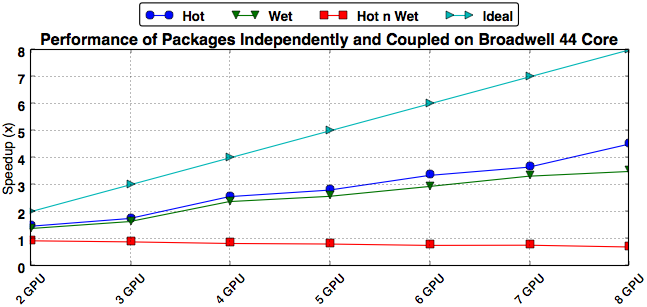
\includegraphics[width=1.0\linewidth]{gpu_storm}
%  \caption{Scaling Hot, Flow, and Hot'n'Flow on a CS STORM node containing 8 NVIDIA K40 GPUs.}
%  \label{fig:scaling-hot-flow-storm}
%\end{figure}
%
%The scaling was generally quite poor on this node and we only achieved a maximum of 50\% efficiency even for the invidual applications. We were surprised to see that the composition of the two applications had lead to some performance bug, which had totally limited scaling on the multi-GPU node.


The results demonstrate that Hot and Flow are performance compatible, meaning they do not interfere with the performance profile of eachother. Although we have not seen a performance degradation at this scale, we think it will be important work to investigate how scaling is affected towards the limits of the scalability of each application.

An interesting feature of the two mini-apps is that they have vastly different performance weightings. For the $5000^2$ problem size, which is a reasonable problem size for realy scientific problems, the capped inner iterations perfomed by \textit{Hot} mean that the performance results shown in Table \ref{tab:hot-flow-multi-device} do not truly represent the imbalance. The true disparity between the runtimes of the two packages is above an order of magnitude. We believe that this has some important implications for the optimisation of the applications when composed. Such an imbalance surely opens up the opportunity for successful overlapping of slow operations...

\subsection{Fast 3d + Hot 3d}

As mentioned throughout the paper, we expected that combining Fast 2d with any of the other mini-apps would lead to conflicts over domain decomposition. For Fast 2d the decomposition ends up being tightly coupled to the resulting algorithm, and in general the literature only suggested one dimensional decompositions for this particular type of problem in 2d. The underlying reason for this decision is that tiling the entire space results in increased inter-process communication. As the parallel FFT algorithm is considered bound by All-to-All communications, this option is therefore deficient.

\subsubsection{Conflict Resolution}

In the event that the data structures within two packages conflict, we can theorise some potential resolutions:

\begin{itemize}
  \item \textbf{Pick the best decomposition for the worst package} - This may or may not be easy depending on the restrictions imposed by the other packages. This is likely only suitable when you have a significant difference between the relative costs of the packages.
  \item \textbf{Choose some mutually beneficial layout} - This could be a complicated decision to make, and might lead to specific novel layouts for particular couplings. If the relative costs of the two packages are similar, then we expect this to be a good choice.
  \item \textbf{Perform a transposition of the data between packages} - Considering a simple two package application, with a victim that requires it's data transposed, this would lead to two transposition at entry to and exit from the victim package. Ideally this transposition could be overlapped with independent work.
\end{itemize}

\section{Patterns Affecting Performance for Multi-Package Applications}

Our research has uncovered a number of areas that we recognise present risks or opportunities to the performance of multi-package applications. 

\begin{itemize}
  \item \textbf{Diverse Computational Weightings} - Each package will expose some fixed or dynamic performance cost for particular problems. We observed with Hot and Flow that the difference in solve times differed by an order of magnitude depending on configuration.
  \item \textbf{Different Optimal Data Layouts} - If choosing an optimal data layout for a package results in a sub-optimal data layout for the other packages, the trade-off is going to be challenging to manage. It is also often the case that applications require different layouts for different architectures, which greatly amplifies this issue. 
  \item \textbf{Competing Decompositions} - It is possible that different packages within an application might require different decompositions for optimal performance. We extend this discussion in Section \ref{sec:scalability-inhibit} to predict a key bottleneck to multi-package scaling.
  \item \textbf{Load Imbalance} - If there is a significant load imbalance in one of the packages the usual approach would be to dynamically adapt the decomposition to re-balance, however when operating in a multi-package environment this will create a load imbalance for the other packages, which will be challenging to handle.
  \item \textbf{Capacity Requirements} - As you increase the number of packages that are included in an application, the capacity requirements can be inflated significantly. It will be important to overlap as much of the capacity as possible in order to minimise this effect. On devices with low capacity, such as accelerator devices, this issue might become a truly limiting factor.
\end{itemize}

We are expecting that continued research into the area of Dwarf composition will begin to uncover some of the points raised above, allowing us to begin tackling the issues.

An important feature of many algorithms that has not yet been acknowledged in this research is the structure of the computational mesh. The Unstructured Grid Dwarf describes those packages that have computational meshes formed of complex graph-based geometries. We are currently deferring the investigation of unstructured meshes, as such a mesh change is in general pervasive. Although it is possible that they exist, our group has never encountered an application that contains solvers for structured \textit{and} unstructured meshes that are intended to be run as part of a multi-package solve.

As the unstructured characteristic greatly increases the complexity of each individual application and would have to be adopted in any applications destined for composition, we will defer this analysis for later investigation.

\subsection{Diminishing Scalability for Increasing Core Counts}

\label{sec:scalability-inhibit}

Modern supercomputing has reached a scale where the core counts at the node level are increasingly significantly each year, and this has major implications for writing portable and performant code. In particular, many of the largest supercomputers in the world include heterogeneous devices, such as accelerators, which greatly increase the core count, and require that significant data-parallelism is exposed within scientific application's algorithms in order to perform well.

Accelerator devices like the Intel Xeon Phi processors, have greater numbers of cores than existing Intel CPUs, for instance the Knights Landing has between 64 and 72, each with 4 hardware threads, whereas the Intel Xeon Broadwell can have up to 22 cores per socket, each core supporting up to 2 hardware threads. The IBM POWER8 CPU also exposes a large thread count, with up to 12 cores per socket and 8 hardware threads for a total of 192 threads.

This continual increase in the number of computational units available on a node has major implications for the scalability of codes, and this is amplified by the increasing number of nodes that are hosting those devices. It is well known that many algorithms reach a turnover point for strong scaling, past which communication costs begin to overwhelm the performance, and decomposing a problem will experience diminishing returns. Regardless of node-level application performance, as communication becomes the limiting factor, we are reaching a stage where the scalability of applications demands that the highly parallel applications exploit shared memory as much as possible.

We predict that it will be particularly important to understand the influence of composing multiple packages on the potential for exploiting local shared memory.

%Extending the discussion to GPGPUs, NVIDIA's Tesla K40 devices have 15 streaming multi-processors (SMX), each of which support 192 processing elements, for a total of 2880 CUDA cores. While those 'CUDA cores' are not cores in the traditional sense, rather individual processing elements, this does not change the fact that any algorithm targeted at these archiectures will need to expose an increasingly large level of parallelism. More recently, NVIDIA released the Tesla P100, which has increased the number of SMXs to 56 and decreased the number of processing elements in each to 64 (two warps), for a total of 3584 CUDA cores.

%The benefit of GPUs is that they offer good performance and can handle significant portions of a problem and require no partitioning within the devices. More recently supercomputing resources have started to include multiple accelerator devices on a single node, and this offers the opportunity for programmers to exploit massive node-level parallelism to improve the scalability of applications. Of course this requires that there is some suitably performant method for communicating within a node. The upcoming NVLINK technology that will be distributed by NVIDIA is intended to provide fast communications between the GPUs on a node and quite improved performance compared to PCIe when communicating with the host CPU. Our expectation is that if this technology can be used to its full extent, it should offer great potential improvements to the scalability of HPC applications. 

%\subsection{Asynchronicity Among Packages}
%
%The balance of different packages within a full application might allow new avenues for overlapping long communications or IO times, or even the potential for overlapping the compute of packages within the full application. We are interested to explore a number of these issues and expect that this could be a future direction for investigation.
%
%The main drawback that we can see with this issue is that overlapping likely complicates the applications so much that it might be possible in the confines of a mini-app, but untenable for a production application. However, if we were to approach this problem, we expect that coarse-grained node-local tasks would be the correct mechanism to support such optimisations.
%
%IF TIME PERMITS WILL ADD SOMETHING TO THIS EFFECT

\section{Future Compositions}

We expect that it will be useful to extend this work to investigate the performance of diverse applications types, in particular we plan to develop new applications that cover the seven Dwarfs of parallel programming. The Bright mini-app hosts a Monte Carlo neutral particle tracking algorithm that we are currently developing. Due to the inherent load imbalance of the problem, it is likely that the application will cause significant performance degradations in general.

Including more applications into the potential compositions leads to many possible combinations. For instance, taking our all four of our current mini-apps we could perform the following coupling:

\begin{figure}
  \centering
  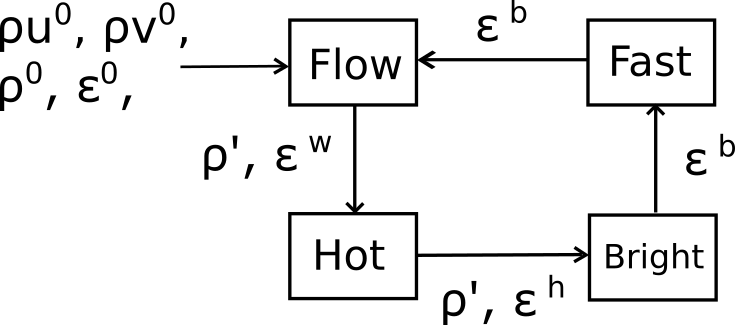
\includegraphics[width=0.6\linewidth]{all-four-flow}
  \caption{The composition of a prospective multi-package application.}
  \label{fig:multi-package-flow}
\end{figure}

We would expect that this sort of package mix could be quite suitable for combustion, or astrophysics (MAKING THAT UP). The resulting performance profile would include lots of all to all communication, several competing decompositions and load imbalance.

\section{Future Work}

We further recognise that there are many requirements not handled by our existing applications, such as multiple materials, complex unstructured geometries, and adaptive mesh refinement. Each of these has a significant influence on the performance of individual algorithms, and likely introduces new issues for coupling packages together. As such it will be essential to consider new mini-apps that can proxy those particular features and consider their performance on new hardware.

\section{Related Work}

(SPEAK TO W ABOUT THIS SECTION, WHAT IS ACCEPTABLE TO BE TIED TO THIS PAPER)

\section{Conclusion}

Although we have only been able to compose three applications in this paper, we have already discovered and discussed some interesting problems that can arise in the process. Importantly we have been able to observe an important fundamental rule with multi-package applications, that the complexity and computational cost of the individual package matters less to the overall performance of the application than the dominant conflicting performance characteristics present amongst the applications.

\bibliographystyle{IEEEtran}
\bibliography{IEEEabrv,multi}

\end{document}

